\documentclass[12pt,english]{article}
\usepackage{authblk}

\usepackage{float}
\usepackage[letterpaper, margin=1in, top=1in, bottom=1in]{geometry}
\usepackage{xcolor}
\usepackage[framemethod=TikZ]{mdframed}
\usepackage{listings}
\usepackage{outlines}
\usepackage{graphicx}
\graphicspath{ {../images/} }
\usepackage{tabularx}
\usepackage{subcaption}
\usepackage{fancyvrb}
\usepackage[english]{babel}
\usepackage{hyperref}

\usepackage{fancyhdr}

\usepackage{amsmath,amsfonts,amssymb,mathrsfs,mathtools}
\usepackage{mathspec}
\DeclarePairedDelimiter\abs{\lvert}{\rvert}%
\DeclarePairedDelimiter\norm{\lVert}{\rVert}%
% Swap the definition of \abs* and \norm*, so that \abs
% and \norm resizes the size of the brackets, and the 
% starred version does not.
\makeatletter
\let\oldabs\abs
\def\abs{\@ifstar{\oldabs}{\oldabs*}}
%
\let\oldnorm\norm
\def\norm{\@ifstar{\oldnorm}{\oldnorm*}}
\makeatother
%%%%%%%%%%%%%%%%%%%

% references for equations
\makeatletter
\def\tagform@#1{\maketag@@@{\bfseries(\ignorespaces#1\unskip\@@italiccorr)}}
\renewcommand{\eqref}[1]{\textup{{\normalfont(\ref{#1}}\normalfont)}}
\makeatother


\usepackage{xparse}

\usepackage{tabto}
\NumTabs{6}

\newcommand{\slide}[2][]{
    \begin{frame}
        \frametitle{
            #1
        }

        #2
    \end{frame}
}

\newcommand{\eq}[2]{
    \begin{equation}\label{#1}
        #2
    \end{equation}
}

\newcommand{\R}{\mathbb{R}}
\newcommand{\Rn}[1][n]{\mathbb{R}^#1}
\NewDocumentCommand{\Rnp}{ O{n} O{p} }{\mathbb{R}^#1_#2}


\renewcommand{\listfigurename}{Figures}

\lstset
{
    language=Python,
    basicstyle=\footnotesize,
    numbers=left,
    numberstyle=\tiny,
    stepnumber=1,
    showstringspaces=false,
    tabsize=1,
    breaklines=true,
    breakatwhitespace=false,
    xleftmargin=-8pt,
    frame=b,
}

\newcommand{\codefile}[3]{
    \mdframed[roundcorner=5pt, backgroundcolor=blue!30]
    \lstinputlisting[caption=$#1$ {#2}, label=#3]{#1}
    \endmdframed
}
\newcommand{\codefilelines}[5]{
    \mdframed[roundcorner=5pt, backgroundcolor=blue!30]
    \lstinputlisting[linerange={#4-#5}, caption=$#1$ Lines #4-#5 {#2}, label=#3]{#1}
    \endmdframed
}
\lstnewenvironment{code}[2]
{
    \mdframed[roundcorner=5pt, backgroundcolor=blue!30]
    \lstset{
        caption={#1},
        label=#2,
    }
}
{
    \endmdframed
}



\title{
    Proposal: A Comparison of Optimization Methods for YOLO Running on Jetson Nano
}
\author{Mark Jeiran}
\author{Igor Semyonov}
\affil{George Mason University}
% \date{}

\begin{document}

\maketitle

\section{Project Summary}

YOLO is a highly capable image detection and classification model.
It has been shown to perform well on various open datasets including coco128, CFAR10, CFAR100, and ImageNet.
An edge device running YOLO could assist in various tasks such as human detection in home security cameras, quality assurance in manufacturing, and obstacle identification in autonomous systems.
We propose to compare compression methods described in \cite{compression-methods} to assess the performance of YOLOv8 on the Jetson Nano platform.
We will write the harness in such a way as to enable easy assessment of deployment to other platforms as well.

\section{ML ALgorithm}

We will use YOLOv5 in this project.
As mentioned earlier, You Only Look Once (YOLO) is a popular object detection model.
The model is well known for its accuracy and efficiency.
\figref{fig:yolo-structure} shows  an overall structure of YOLO v5 as shown in Figure 1:

\begin{figure}[h]
    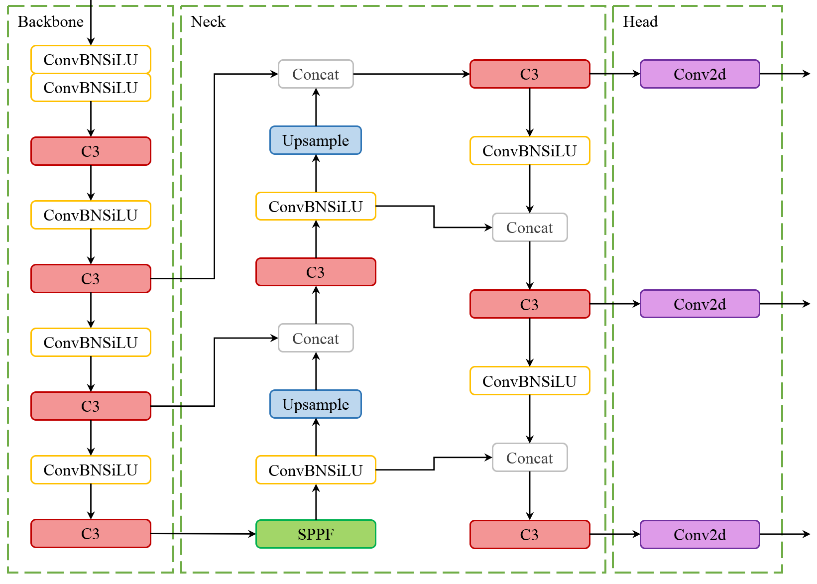
\includegraphics[width=0.8\linewidth]{yolo-structure}
    \caption{YOLOv5 architecture \cite{compression-methods}}
    \label{fig:yolo-structure}
\end{figure}

Backbone: YOLO v5 supports various backbone architectures.
The backbone is a convolutional neural network (CNN), which acts as a feature extractor from the input image.

Detection Neck: Features extracted from the backbone are fed into the neck, which further process them.
Feature fusion, dimensionality reduction, and spatial aggregation are often used to enhance the representation of features.

Detection Head: Detection head as the last layer is comprised of convolutional layers to predict bounding boxes and class probabilities.
Typically, each predicted bounding box includes coordinates (x, y) for the box's center, width, and height, along with confidence scores for object presence and class probabilities.

\section{Target Platform}

Jetson Nano (16GB).
NVIDIA Jetson Nano is a low-cost AI computer.
It delivers the compute performance to run modern AI workloads at unprecedented size.
It is incredibly power-efficient, consuming as little as 5 watts.

\section{Optimization Approach}

We will train the model using a desktop workstation with a GPU.
The model will be optimized using Quantization-Aware Training (QAT) and Post-Training Quantization (PTQ) methods.
QAT is the quantization of a pre-trained model then finetuning using training data to improve accuracy.
The calibration process frequently occurs concurrently with the finetuning process in QAT.
However, in PTQ a pre-trained model is calibrated using as a small subset of training data, to determine clipping ranges and scaling factors, then the model is quantized according to the calibration outcomes [2].
The primary difference in the methodology of these two methods is illustrated in \figref{fig:ptq-vs-qat}.

\begin{figure}[h]
    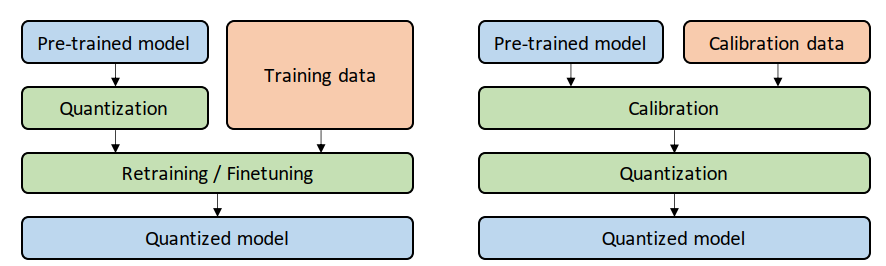
\includegraphics[width=0.8\linewidth]{ptq-vs-qat}
    \caption{PTQ vs QAT quantization process comparison \cite{quantization-methods}}
    \label{fig:ptq-vs-qat}
\end{figure}

\section{Metrics}

We will evaluate the efficacy of our compression methods using GFLOPS vs Accuracy and number of Parameters vs Accuracy.
We will also use the coco metrics of mean average precision (mAP) in both @0.5 and @0.95 variants as evaluation metrics.

\section{Dataset}

We will use CFAR100 as the train and test set.
CIFAR100 has 60,000 32x32 color images in 100 classes, with 600 images per class.
These images are split into 50,000 training images and 10,000 test images.

%\section*{References}
% \nocite{hybrid-sparcity}
\bibliographystyle{siam}
\bibliography{refs}

%\layout*

\end{document}
